% ========================================
%	Header einbinden
% ========================================

\documentclass[bibtotoc,titlepage]{scrartcl}

% Deutsche Spracheinstellungen
\usepackage[ngerman,german]{babel, varioref}
\usepackage[T1]{fontenc}
\usepackage[utf8]{inputenc}

%\usepackage{marvosym}

\usepackage{amsfonts}
\usepackage{amssymb}
\usepackage{amsmath}
\usepackage{amscd}
\usepackage{amstext}

\usepackage{longtable}

%\usepackage{bibgerm}

\usepackage{footnpag}

\usepackage{ifthen}                 %%% package for conditionals in TeX
\usepackage[amssymb]{SIunits}
%Für textumflossene Bilder und Tablellen
%\usepackage{floatflt} - veraltet

%Für Testzwecke aktivieren, zeigt labels und refs im Text an.
%\usepackage{showkeys}

% Abstand zwischen zwei Absätzen nach DIN (1,5 Zeilen)
% \setlength{\parskip}{1.5ex plus0.5ex minus0.5ex}

% Einrückung am Anfang eines neuen Absatzes nach DIN (keine)
%\setlength{\parindent}{0pt}

% Ränder definieren
% \setlength{\oddsidemargin}{0.3cm}
% \setlength{\textwidth}{15.6cm}

% bessere Bildunterschriften
%\usepackage[center]{caption2}


% Problemlösungen beim Umgang mit Gleitumgebungen
\usepackage{float}

% Nummeriert bis zur Strukturstufe 3 (also <section>, <subsection> und <subsubsection>)
%\setcounter{secnumdepth}{3}

% Führt das Inhaltsverzeichnis bis zur Strukturstufe 3
%\setcounter{tocdepth}{3}
\usepackage[version=3]{mhchem}
	\mhchemoptions{minus-sidebearing-left=0.06em, minus-sidebearing-right=0.11em}
\usepackage{exscale}

\newenvironment{dsm} {\begin{displaymath}} {\end{displaymath}}
\newenvironment{vars} {\begin{center}\scriptsize} {\normalsize \end{center}}


\newcommand {\en} {\varepsilon_0}               % Epsilon-Null aus der Elektrodynamik
\newcommand {\lap} {\; \mathbf{\Delta}}         % Laplace-Operator
\newcommand {\R} { \mathbb{R} }                 % Menge der reellen Zahlen
\newcommand {\e} { \ \mathbf{e} }               % Eulersche Zahl
\renewcommand {\i} { \mathbf{i} }               % komplexe Zahl i
\newcommand {\N} { \mathbb{N} }                 % Menge der nat. Zahlen
\newcommand {\C} { \mathbb{C} }                 % Menge der kompl. Zahlen
\newcommand {\Z} { \mathbb{Z} }                 % Menge der kompl. Zahlen
\newcommand {\limi}[1]{\lim_{#1 \rightarrow \infty}} % Limes unendlich
\newcommand {\sumi}[1]{\sum_{#1=0}^\infty}
\newcommand {\rot} {\; \mathrm{rot} \,}         % Rotation
\newcommand {\grad} {\; \mathrm{grad} \,}       % Gradient
\newcommand {\dive} {\; \mathrm{div} \,}        % Divergenz
\newcommand {\dx} {\; \mathrm{d} }              % Differential d
\newcommand {\cotanh} {\; \mathrm{cotanh} \,}   %Cotangenshyperbolicus
\newcommand {\asinh} {\; \mathrm{areasinh} \,}  %Area-Sinus-Hyp.
\newcommand {\acosh} {\; \mathrm{areacosh} \,}  %Area-Cosinus-H.
\newcommand {\atanh} {\; \mathrm{areatanh} \,}  %Area Tangens-H.
\newcommand {\acoth} {\; \mathrm{areacoth} \,}  % Area-cotangens
\newcommand {\Sp} {\; \mathrm{Sp} \,}
\newcommand {\mbe} {\stackrel{\text{!}}{=}}     %Must Be Equal
\newcommand{\qed} { \hfill $\square$\\}
\renewcommand{\i} {\imath}
\def\captionsngerman{\def\figurename{\textbf{Abb.}}}

%%%%%%%%%%%%%%%%%%%%%%%%%%%%%%%%%%%%%%%%%%%%%%%%%%%%%%%%%%%%%%%%%%%%%%%%%%%%
% SWITCH FOR PDFLATEX or LATEX
%%%%%%%%%%%%%%%%%%%%%%%%%%%%%%%%%%%%%%%%%%%%%%%%%%%%%%%%%%%%%%%%%%%%%%%%%%%%
%%%
\ifx\pdfoutput\undefined %%%%%%%%%%%%%%%%%%%%%%%%%%%%%%%%%%%%%%%%% LATEX %%%
%%%
\usepackage[dvips]{graphicx}       %%% graphics for dvips
\DeclareGraphicsExtensions{.eps,.ps}   %%% standard extension for included graphics
\usepackage[ps2pdf]{thumbpdf}      %%% thumbnails for ps2pdf
\usepackage[ps2pdf,                %%% hyper-references for ps2pdf
bookmarks=true,%                   %%% generate bookmarks ...
bookmarksnumbered=true,%           %%% ... with numbers
hypertexnames=false,%              %%% needed for correct links to figures !!!
breaklinks=true,%                  %%% breaks lines, but links are very small
linkbordercolor={0 0 1},%          %%% blue frames around links
pdfborder={0 0 112.0}]{hyperref}%  %%% border-width of frames
%                                      will be multiplied with 0.009 by ps2pdf
%
\hypersetup{ pdfauthor   = {Hannes Franke; Julius Tilly},
pdftitle    = {V301 Innenwiderstand und Leistungsanpassung}, pdfsubject  = {Protokoll FP}, pdfkeywords = {V301, Innenwiderstand, Leistungsanpassung},
pdfcreator  = {LaTeX with hyperref package}, pdfproducer = {dvips
+ ps2pdf} }
%%%
\else %%%%%%%%%%%%%%%%%%%%%%%%%%%%%%%%%%%%%%%%%%%%%%%%%%%%%%%%%% PDFLATEX %%%
%%%
\usepackage[pdftex]{graphicx}      %%% graphics for pdfLaTeX
\DeclareGraphicsExtensions{.pdf}   %%% standard extension for included graphics
\usepackage[pdftex]{thumbpdf}      %%% thumbnails for pdflatex
\usepackage[pdftex,                %%% hyper-references for pdflatex
bookmarks=true,%                   %%% generate bookmarks ...
bookmarksnumbered=true,%           %%% ... with numbers
hypertexnames=false,%              %%% needed for correct links to figures !!!
breaklinks=true,%                  %%% break links if exceeding a single line
linkbordercolor={0 0 1},
linktocpage]{hyperref} %%% blue frames around links
%                                  %%% pdfborder={0 0 1} is the default
\hypersetup{
pdftitle    = {V301 Innenwiderstand und Leistungsanpassung}, 
pdfsubject  = {Protokoll AP}, 
pdfkeywords = {V301, Innenwiderstand, Leistungsanpassung},
pdfsubject  = {Protokoll AP},
pdfkeywords = {V301, Innenwiderstand, Leistungsanpassung}}
%                                  %%% pdfcreator, pdfproducer,
%                                      and CreationDate are automatically set
%                                      by pdflatex !!!
\pdfadjustspacing=1                %%% force LaTeX-like character spacing
\usepackage{epstopdf}
%
\fi %%%%%%%%%%%%%%%%%%%%%%%%%%%%%%%%%%%%%%%%%%%%%%%%%%% END OF CONDITION %%%
%%%%%%%%%%%%%%%%%%%%%%%%%%%%%%%%%%%%%%%%%%%%%%%%%%%%%%%%%%%%%%%%%%%%%%%%%%%%
% seitliche Tabellen und Abbildungen
%\usepackage{rotating}
\usepackage{ae}
\usepackage{
  array,
  booktabs,
  dcolumn
}
\makeatletter 
  \renewenvironment{figure}[1][] {% 
    \ifthenelse{\equal{#1}{}}{% 
      \@float{figure} 
    }{% 
      \@float{figure}[#1]% 
    }% 
    \centering 
  }{% 
    \end@float 
  } 
  \makeatother 


  \makeatletter 
  \renewenvironment{table}[1][] {% 
    \ifthenelse{\equal{#1}{}}{% 
      \@float{table} 
    }{% 
      \@float{table}[#1]% 
    }% 
    \centering 
  }{% 
    \end@float 
  } 
  \makeatother 
%\usepackage{listings}
%\lstloadlanguages{[Visual]Basic}
%\allowdisplaybreaks[1]
%\usepackage{hycap}
%\usepackage{fancyunits}

\usepackage{float}
\usepackage{caption}
\usepackage{wrapfig}
\usepackage{setspace}
\usepackage{threeparttable}
\usepackage{footnote}

\newfloat{formel}{htbp}{for}
\floatname{formel}{Formel}

% ========================================
%	Angaben für das Titelblatt
% ========================================

\title{Das Kugelfall Viskosimeter nach Höppler\\				% Titel des Versuchs 
\large TU Dortmund, Fakultät Physik\\ 
\normalsize Anfänger-Praktikum}

\author{Jan Adam\\			% Name Praktikumspartner A
{\small \href{jan.adam@tu-dortmund.de}{jan.adam@tu-dortmund.de}}	% Erzeugt interaktiven einen Link
\and						% um einen weiteren Author hinzuzfügen
Dimitrios Skodras\\			% Name Praktikumspartner B
{\small \href{dimitrios.skodras@tu-dortmund.de}{dimitrios.skodras@tu-dortmund.de}}		% Erzeugt einen interaktiven Link
}
\date{04.12.12}					% Das Datum der Versuchsdurchführung

% ========================================
%	Das Dokument beginnt
% ========================================

\begin{document}

% ========================================
%	Titelblatt erzeugen
% ========================================

\maketitle					% Jetzt wird die Titelseite erzeugt
\thispagestyle{empty} 				% Weder Kopfzeile noch Fußzeile

% ========================================
%	Der Vorspann
% ========================================

%\newpage					% Wenn Verzeichnisse auf einer neuen Seite beginnen sollen
%\pagestyle{empty}				% Weder Kopf- noch Fußzeile für Verzeichnisse

\tableofcontents

%\newpage					% eine neue Seite
%\thispagestyle{empty}				% Weder Kopf- noch Fußzeile für Verzeichnisse
%\listoffigures					% Abbildungsverzeichnis

%\newpage					% eine neue Seite
%\thispagestyle{empty}				% Weder Kopf- noch Fußzeile für Verzeichnisse
%\listoftables					% Tabellenverzeichnis
\newpage					% eine neue Seite


% ========================================
%	Kapitel
% ========================================

%	\section{Einleitung}				% Bei Bedarf

	\section{Theorie}
Auf bewegte Körper in Flüssigkeiten oder Gasen wirkt, ähnlich wie auf rollende oder gleitende Körper, eine Reibungskraft
\begin{align}
\vec F_R=-6 \pi \eta \vec{v} r,
\label{stokes}
\end{align}
 die der Bewegung entgegen wirkt. Wichtig ist hier die Viskosität $\eta $, eine Stoffeigenschaft, die das Fließverhalten von Flüssigkeiten und Gasen beschreibt und proportional auf die Reibungskraft einwirkt. Sie ist zudem die einzige stoffspezifische Größe, die Einfluss auf die Reibungskraft hat. 
$\eta$ errechnet sich über
\begin{equation}
  \eta = K(\rho_K - \rho_{Fl})\cdot t.
  \label{viskos}
 \end{equation}
Dabei ist K die Apparaturkonstante, welcher jene Geometriegrößen, sowie die Fallhöhe enthält. t entspricht der gemessenen Fallzeit und $\rho_K$ und $\rho_{Fl}$ der Kugel- bzw. der Flüssigkeitsdichte.
Die restlichen Größen hängen lediglich von der Körpergeometrie ab, sodass man die Viskosität mit der oben angegebenen Formel ermitteln lässt. 

 Zu beachten ist, dass die durch Gleichung \eqref{stokes} beschriebene Stokes'sche Reibung nur für laminare Flüssigkeiten gilt. Laminare Flüssigkeiten bilden keine Verwirbelungen, sondern umfließen den Körper homogen. Eine Flüssigkeit wird als laminar bezeichnet, wenn ihre Reynoldszahl
 \begin{align}
 Re= \frac{\rho v d}{\eta} = \frac{v d}{\nu}
 \label{rey}
 \end{align}
unter dem kritischen Wert von 2040 \footnote{Quelle: \href{http://homepages.warwick.ac.uk/~masax/Research/critical_point_pipe_flow/critical_point_pipe_flow.html}{http://homepages.warwick.ac.uk} } bleibt. Ab diesem Wert werden Flüssigkeiten nicht mehr als laminar bezeichnet, jedoch können sich Verwirbelungen schon viel früher bilden, so dass  $Re \ll 2040$ sein sollte. 
	\section{Aufbau}
\begin{wrapfigure}[11]{r}{3.5cm}
	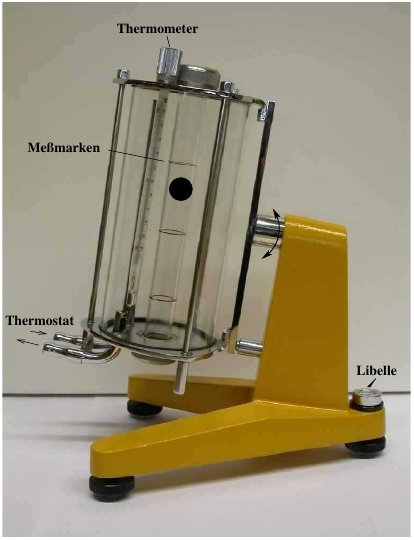
\includegraphics[width=0.23\textwidth]{pics/aufbau.jpg}
	\caption{Viskosimeter}
	\label{aufbau}
\end{wrapfigure}

Beim Kugelfall-Viskosimeters nach Höppler handelt es sich um zwei ineinander eingelassene Hohlzylinder aus Glas, welche mit Flüssigkeiten befüllt und hermetisch abgeschlossen werden können. Auf Abbildung \ref{aufbau} \footnote{Viskosimeter nach Höppler - Das Bild ist aus der Versuchsanleitung entnommen} ist das Viskosimeter zu erkennen.\\
Der innere Zylinder weißt Markierunge auf, durch die eine Strecke von $x$ = 10 cm abgemessen wird. Er wird während des Versuchs mit der Flüssigkeit befüllt, deren Viskosität bestimmt werden soll. Dazu legt man eine Kugel hinein, deren Durchmesser nur geringfügig kleiner ist, als der des Zylinders. An einem Schanier kann man das Viskosimeter vertikal drehen, so dass die Kugel abzusinken beginnt. Durch das Messen der Zeit, die die Kugel benötigt um die Markierungen zu passieren kann man errechnen, welche Geschwindigkeit die Kugel erreicht.\\
Beim Fallen wirken folgende Kräfte auf die Kugel: die Gewichtskraft $F_g$, die die Kugel nach unten beschleunigt, die Auftriebskraft $F_A$, die die Kugel nach oben treibt und die Reibungskraft \eqref{stokes}, die proportional zur Fallgeschwindigkeit ist und ihr entgegen wirkt. Nach dem Fallenlassen nimmt die Geschwindigkeit der Kugel zunächst immer weiter zu, bis sich schließlich durch Zunahme der Reibungskraft ein Kräftegleichgewicht einstellt und die Kugel mit konstanter Geschwindigkeit absinkt.\\
Über ein Thermometer wird dabei abgelesen, welche Temperatur die Probe zur Zeit hat und mit einer Libelle wird sichergestellt, dass das Viskosimeter im richtigen Winkel steht.\\
Der äußere Zylinder hat zwei Anschlüsse, durch die temperiertes Wasser fließen kann und somit die Temperatur der Probe veränderbar wird. Dies ist wichtig, da die Viskosität stark Temperaturabhängig ist und so eine Temperaturabhängigkeit dargestellt werden kann. 

	\section{Durchführung}
Im durchgeführten Versuch soll die Viskosität von destillierem Wasser mit Hilfe des Kugelfall-Viskosimeters nach Höppler bestimmt werden. Dabei wird eine Kugel in einen mit destilliertem Wasser gefüllten Zylinder gelegt und dieser so aufgestellt, dass die Kugel hindurchfällt. Wichtig ist dabei, dass der Kugeldurchmesser nur geringfügig kleiner ist als der des Zylinders und dass dieser leicht geneigt ist, damit die Kugel nicht chaotisch an die Ränder stößt und Wirbel verursacht, sondern gleichmäßig herabgleitet.\\
Sobald die Kugel gleichmäßig absinkt wird die Zeit gemessen, die die Kugel braucht um eine Strecke $d = 10cm$ zurückzulegen. Hieraus lässt sich die Geschwindigkeit der Kugel und schließlich mit Gleichung \eqref{viskos} die Viskosität des Wassers errechnen.\\
Der Versuch wird zweimal bei Raumtemperatur mit verschiedenen Kugeln und dann mit nur einer Kugel bei verschiedenen Wassertemperaturen von $20 ^\circ $ bis $50 ^\circ $ C durchgeführt, da die Viskosität stark von der Temperatur abhängig ist. Halblogarithmisches Auftragen der Daten ermöglicht ein Ablesen der Konstanten A und B aus der Andradeschen Gleichung
\begin{align}
	\eta(T)=Ae^{\left(\frac{B}{T}\right)},
	\label{andrade}
\end{align}
welche die Viskosität in Abhängigkeit von der Temperatur beschreibt.

\section{Auswertung}
\subsection{Fehlerrechnung}
Da viele für die Auswertung notwendigen Größen fehlerbehaftet sind, ist es wichtig, den Einfluss dieser Fehler auf die ermittelten
Größen herauszufinden. Neben den, von den Messapparaturen verursachten Fehlern, dienen der Mittelwert
\newpage
\begin{formel}
\begin{equation}
 \bar{x} = \frac1N \sum_{i=1}^{N} x_i,
\end{equation}
\caption*{\small{$\bar{x}$ = Mittelwert, N = Anzahl der Messungen}}
\end{formel}

die Gaußsche Fehlerfortpflanzung

\begin{formel}
\begin{equation}
\Delta G = \sqrt{\sum_{i=1}^{N}\left( \frac{\partial G}{\partial x_i}\cdot \Delta x_i\right)^2},
\label{gauss}
\end{equation}
\caption*{$x_i$ = Variable, $\Delta x_i$ = Fehler der Variable}
\end{formel}

und die Standardabweichung des Mittelwerts

\begin{equation}
 \bar s = \sqrt{\frac{1}{N(N-1)} \sum_{i}^{N} (x_i - \bar{x})^2}.
\end{equation}

\subsection{Viskosität des Wassers}

\renewcommand{\arraystretch}{1.2}
\begin{table}[h]
 \begin{tabular}{c|c||c|c}
 t$_{kl}$[s] & t$_{kl}$[s] Forts. & t$_{gr}$[s] & t$_{gr}$[s] Forts.\\
 \hline
12,42&	12,01&	71,10&	71,13\\
12,30&	12,30&	71,00&	71,56\\
11,98&	11,95&	71,35&	70,93\\
12,30&	11,89&	71,52&	71,43\\
12,10&	11,90&	71,38&	70,90\\
12,03&	12,20&	71,32&	71,10\\
12,02&	12,23&	71,18&	71,06\\
11,79&	12,15&	71,03&	71,90\\
11,98&	11,92&	70,96&	71,21\\
11,88&	12,09&	71,05&	71,36\\
\hline
$\bar t_{kl}$[s] &12,072 &$\bar t_{gr}[s] $&71,223\\
$\bar s_{kl}$[s] & 0,039 & $\bar s_{gr}$[s] & 0,057
 \end{tabular}
\caption{Messzeiten für beide Kugeln durch das Fallrohr}
\label{tabviskos}
\end{table}
\renewcommand{\arraystretch}{1}

Zur Ermittlung der Viskosität wird Formel \eqref{viskos} verwandt. Der Versuch wird mit zwei verschiedenen Kugeln durchgeführt, wobei
für eine die Apparaturkonstante $K_{kl}$ bekannt ist. Mit der ebenfalls gegebenen Masse der kleinen Kugel, sowie ihrem gemessenen Durchmesser
lässt sich die Dichte $\rho_{kl}$ ermitteln. Die Dichte von Wasser wird aus Literaturangaben entnommen. Um die Apparaturkonstante 
$K_{gr}$ zu bestimmen, sind neben der errechneten Viskosität die Dichte $\rho_{gr}$ aus gemessenem Durchmesser und gemessener Masse nötig.


Der Fehler der Durchmesser d$_{kl/gr}$ wird durch den auf der Schieblehre angegebene Fehler verwandt. Jener Fehler der Massen m$_{kl/gr}$
entspricht der kleinsten Größenordnung der zur Messung benutzten Waage. Die Dichte von Wasser als benötigter Wert wurde aus
({wissenschaft-technik-ethik.de von Dr.-Ing H. Grimm, Wasser und Dichte/Dichtetabelle - URL: \href{http://www.wissenschaft-technik-ethik.de/wasser_dichte.html#kap02}{www.wissenschaft-technik-ethik.de/wasser\_dichte.html}})
entnommen. Die Fehler der Dichten $\rho_{kl/gr}$ ergeben sich aus \eqref{gauss} zu

\begin{align}
  \nonumber
  \Delta \rho_{kl} &= \sqrt{\left(\frac{\partial \rho_{kl}}{\partial d_{kl}} \Delta d_{kl}\right)^2  + \left(\frac{\partial \rho_{kl} }{\partial m_{kl} } \Delta m_{kl}\right)^2 } = \rho_{kl} \sqrt{\left(-3\frac{\Delta d_{kl}}{d}\right)^2+\left(\frac{\Delta m_{kl}}{m}\right)^2} \\
  &= 0,014 \frac{g}{cm^3}\\
  \nonumber
  \Delta \rho_{gr} &= \sqrt{\left(\frac{\partial \rho_{gr}}{\partial d_{gr}} \Delta d_{gr}\right)^2  + \left(\frac{\partial \rho_{gr} }{\partial m_{gr} } \Delta m_{gr}\right)^2 } = \rho_{gr} \sqrt{\left(-3\frac{\Delta d_{gr}}{d}\right)^2+\left(\frac{\Delta m_{gr}}{m}\right)^2} \\
  &= 0,074 \frac{g}{cm^3} \quad \text{mit} \quad\rho = \frac{m}{\frac16 \pi d^3}
  \label{dichte}
\end{align}

\begin{table}[h]
 \begin{tabular}{l|l|l}
 Größe & Wert & Fehler\\
 \hline
  $d_{kl}$ & 13,7 mm & 0,02 mm\\
  $d_{gr}$ & 13,8 mm & 0,02 mm\\
\hline
  $m_{kl}$ & 4,4531 g & - \\
  $m_{gr}$ & 5,0 g & 0,1 g\\
\hline
  $\rho_{kl}$ & 3,308 $\frac{\text{g}}{\text{cm$^3$}}$& 0,014 $\frac{\text{g}}{\text{cm$^3$}}$ \\
  $\rho_{gr}$ & 3,634 $\frac{\text{g}}{\text{cm$^3$}}$& 0,074 $\frac{\text{g}}{\text{cm$^3$}}$ \\
  $\rho_{Fl}$ & 0,998 $\frac{\text{g}}{\text{cm$^3$}}$& - \\
  \hline
$K_{kl}$ & 0,07640 $\frac{\text{mPa}\cdot\text{cm}^3}{\text{g}}$ & -
 \end{tabular}
\caption{relevante Kenngrößen}
\end{table}

Aus den nun bekannten Größen ermittelt sich $\eta$ mit dem Fehler aus \eqref{gauss} zu

\begin{align}
 \nonumber
 \eta = K_{kl}(\rho_{kl}-\rho_{Fl}) \bar t_{kl} &= 0,07640 \frac{\text{mPa}\cdot\text{cm}^3}{\text{g}} \cdot \left(3,308\frac{\text{g}}{\text{cm$^3$}} - 0,998 \frac{\text{g}}{\text{cm$^3$}}\right)\cdot 12,072 \text{s}\\
 &= 2,131 \text{mPas}
\end{align}
\begin{align}
\nonumber
 \Delta \eta &= \sqrt{\left(\frac{\partial \eta}{\partial \rho_{kl}}\Delta \rho_{kl}\right)^2 + \left(\frac{\partial \eta}{\partial t} \bar s_{kl}\right)^2} = \eta \sqrt{\left(\frac{\Delta \rho_{kl}}{(\rho_{kl}-\rho_{Fl})}\right)^2 + \left(\frac{\bar s_{kl}}{t}\right)^2} \\
 &= 0,015 \text{mPas}
\end{align}

Die gesuchte Apparaturkonstante $K_{gr}$ lässt sich nun errechnen durch Gleichsetzen:

\begin{align}
 \nonumber
 K_{gr}(\rho_{gr} - \rho_{Fl})\cdot t_{gr} &= K_{kl}(\rho_{kl} - \rho_{Fl})\cdot t_{kl} \Leftrightarrow K_{gr} = K_{kl}\frac{(\rho_{kl} - \rho_{Fl})}{(\rho_{gr} - \rho_{Fl})}\cdot\frac{t_{kl}}{t_{gr}}\\
 &K_{gr} = 0,01135\, \frac{\text{mPa}\cdot\text{cm}^3}{\text{g}}
\end{align}
\begin{align}
 \nonumber
\Delta K_{gr} &= \sqrt{\left(\frac{\partial K_{gr}}{\partial \rho_{kl}}\Delta \rho_{kl} \right)^2 + \left(\frac{\partial K_{gr}}{\partial \rho_{gr}}\Delta \rho_{gr} \right)^2 + \left(\frac{\partial K_{gr}}{\partial t_{kl}} \bar s_{kl} \right)^2 + \left(\frac{\partial K_{gr}}{\partial t_{gr}} \bar s_{gr} \right)^2}\\
 \nonumber
 &= K_{gr} \sqrt{\left(\frac{\Delta \rho_{kl}}{(\rho_{kl}-\rho_{Fl})} \right)^2 + \left(-\frac{\Delta \rho_{gl}}{(\rho_{gl}-\rho_{Fl}} \right)^2 + \left(\frac{\bar s_{kl}}{t} \right)^2 + \left(\frac{\bar s_{gr}}{t} \right)^2}\\
 &= 0,00033 \, \frac{\text{mPa}\cdot\text{cm}^3}{\text{g}}
\end{align}

<<<<<<< HEAD
=======

Um die Verwendung genannter Formeln zur Ermittlung der Viskosität zu rechtfertigen, muss die Reynoldszahl für diesen Versuch ermittelt und mit 
der kritischen Reynoldszahl verglichen werden. Nach \eqref{rey} ergibt sich

\begin{equation}
 Re = \frac{d_{kl}\cdot \rho_{Fl}}{\eta} \cdot \frac{x}{t_{kl}}=\frac{998\frac{\text{kg}}{\text{m}^3} \cdot 0,00828\frac{\text{m}}{\text{s}} \cdot 0,0137 \text{m}}{0,002313 \text{Pa}\cdot\text{s}} \approx 49 \ll 2040,
\end{equation}

weshalb man von einer laminaren Flüssigkeit sprechen darf und das Verwenden der Formeln legitim ist.

>>>>>>> 3a1143facea85f731a95290d96da519a3fa42f86
\subsection{Anwendung der Andrade-Gleichung}
Um die Koeffizienten A und B aus Gleichung \eqref{andrade} zu ermitteln, wird die Fallzeit zu verschiedenen Temperaturen gemessen.

\renewcommand{\arraystretch}{1.2}
\begin{table}[H]
 \begin{tabular}{c|c|c|c|c}
   T [K] & $\frac{1}{\text{T}}[\frac{1}{\text{K}}]$& $t_1$ [s] & $t_2$[s] & ln($\frac{\eta}{\text{mPas}}$)\\	
   \hline
294	&0,00340&	81,16&	81,04&	0,88 \\
299&	0,00334&	72,87&	72,92&	0,78\\
302&	0,00331&	68,27&	68,41&	0,71\\
305&	0,00328	&64,44&	64,15&	0,65\\
308&	0,00325	&60,41&	60,69&	0,59\\
311&	0,00321&	57,61&	57,55&	0,54\\
314&	0,00318&	54,61&	54,04&	0,48\\
317&	0,00315&	51,32&	51,83&	0,43\\
320&	0,00312&	49,00&	49,24&	0,38\\
323&	0,00309&	46,58&	46,24&	0,32\\
326&	0,00307&	44,47&	44,80&	0,29\\

 \end{tabular}
\caption{Durch Temperaturerhöhung verringerte Fallzeit}
\label{tabandrade}
\end{table}
\renewcommand{\arraystretch}{1}

Um aus dem Exponentialzusammenhang eine lineare Beziehung herzustellen, werden folgende Umformungsschritte unternommen, damit dann durch lineare Regression mittels GNUplot
die Koeffizienten bestimmt werden können:

\begin{align*}
 \eta(T) &= A \exp \left(\frac{B}{T}\right) \\
 \underbrace{\ln \left( \frac{\eta}{\text{mPas}} \right)}_{=y} &= \underbrace{\frac{B}{T}}_{=a\cdot x} +  \underbrace{\ln(A) }_{=b}
\end{align*}

\begin{equation}
\text{mit } a = 1783,92\pm 25,4 \quad \text{und} \quad b = -5,19 \pm 0,08.\\
\end{equation}

Zurücktransferiert erhält man wieder A und B zu

\begin{align}
 A = \e^b &= 5,57 \cdot 10^{-3} \pm 4,46 \cdot 10^{-4}\\
 B = a &= 1783,92 \pm 25,4
\end{align}

\begin{table}[H]
 \begin{tabular}{c|c|c|c|c|c|c|c|c|c|c|c}
  $T$ in $K$ & 294 & 299 & 302 & 305 & 308 & 311 & 314 & 317 & 320 & 323 & 326 \\
  \hline
  $Re$ & 7,0 &	8,6	&9,7	&10,9	&12,3	&13,6	&15,3	&17,0	&18,8	&20,9	&22,9
 \end{tabular}
\caption{Legitimierung der verwandten Formeln mit Reynoldszahlen weit unter 2040}
\end{table}


\begin{figure}[H]
%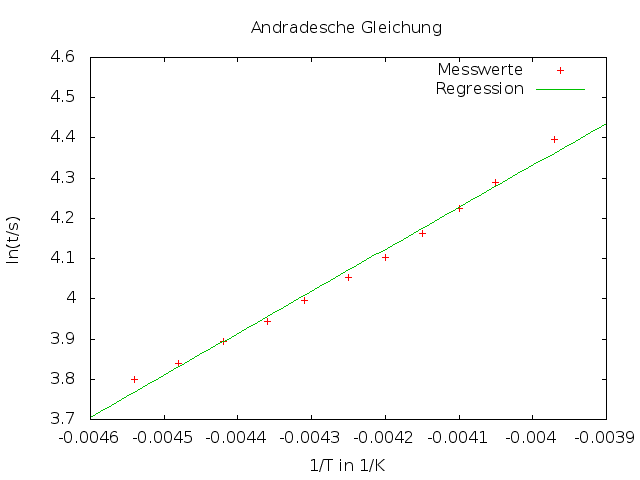
\includegraphics[width=0.7\textwidth] {pics/Andrade.pdf}
\centering
\caption{lineare Abhängigkeit von $\frac1T$ und ln($\frac{\eta}{\text{mPas}}$)}
\end{figure}

\begin{figure}[H]
%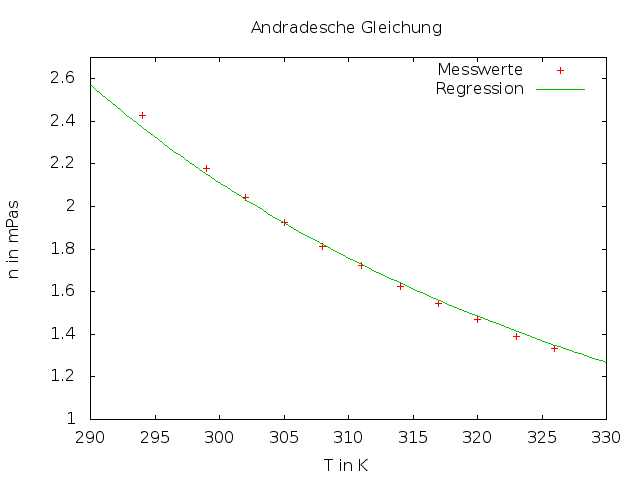
\includegraphics[width=0.7\textwidth] {pics/Viskos.pdf}
\centering
\caption{endgültige Andrade-Gleichung}
\end{figure}

\section{Diskussion}
Im Vergleich zu Referenzwerten ({wissenschaft-technik-ethik.de von Dr.-Ing H. Grimm, Eigenschaften von Wasser - URL: \href{http://www.wissenschaft-technik-ethik.de/wasser_eigenschaften.html#kap06}{www.wissenschaft-technik-ethik.de/wasser\_eigenschaften.html}})
stellt sich heraus, dass die ermittelte Viskosität von 

\begin{align*}
 \eta = 2,131 \text{mPas} \pm 0,015 \text{mPas}
\end{align*}

um mehr als das doppelte abweicht. Da sie durch Gleichung \eqref{viskos} ermittelt wird, sind nur zwei Fehlerquellen möglich. Zum einen
die Dichte der kleinen Kugel $\rho_{kl}$, sowie die Zeit $t_{kl}$. Da die benötigte Zeit 20 Mal gemessen wurde, fällt sie als Ursache
wahrscheinlich aus. Somit bleibt die Dichte, die aus der gegebenen Masse $m_{kl}$ und dem gemessenen Durchmesser $d_{kl}$ nach \eqref{dichte}
zusammengesetzt ist. Nach dem Durchmesser aufgelöst ergibt sich

\begin{align}
  \nonumber
  d &= \sqrt[3]{\frac{6\, m_{kl} \, K_{kl} \, t_{kl} }{\pi \left(\eta + \rho_{Fl} \, K_{kl} \, t_{kl}\right)}} = \sqrt[3]{\frac{6\cdot 4,4531 \text{g} \cdot 0,0764 \,\frac{\text{mPas}\cdot \text{cm}^3}{\text{g}} \cdot 12,072 \,\text{s} }{\pi \left(1\,\text{mPas} + 0,998  \frac{\text{g}}{\text{cm}^3} \cdot 0,0764 \,\frac{\text{mPas}\cdot \text{cm}^3}{\text{g}} \cdot 12,072 \,\text{s}\right)}}\\
  &= 16,0 \text{mm} \neq 13,7 \text{mm},
\end{align}

was eine Messungenauigkeit von 2,3 mm (14,4 \%) bedeutet.

Desweiteren ist es auffällig, dass die zur Ermittlung der Apparaturkonstante gemessene Zeit $t_{gr}$ in Tabelle \ref{tabviskos} um etwa zehn 
Sekunden von der Messung von $t$ aus Tabelle \ref{tabandrade} bei gleicher Temperatur von 21 $^\circ$C abweicht. 
Es handelt sich hierbei um einen systematischen Fehler. Möglicherweise ist die Versuchskugel beim Wechsel der Kugel im Viskosimeter 
versehentlich verwechselt worden.


% ========================================
%	Literaturverzeichnis
% ========================================

%\bibliographystyle{plainnat}			% Bibliographie-Style auswählen
%\bibliography{BIBDATEI}			% Literaturverzeichnis

% ========================================
%	Das Dokument endent
% ========================================

\end{document}
